\documentclass{article}
\usepackage[T1]{fontenc}
\usepackage{enumerate}
\usepackage[fleqn]{mathtools}
\usepackage{multicol}
\usepackage{amssymb}
\usepackage[margin=0.75in, bottom=1in]{geometry}
\usepackage{glossaries}
\usepackage{float}
\usepackage{xcolor}
\usepackage{tabularx}
\usepackage{hyperref}
\hypersetup{
    colorlinks=true,
    allcolors=blue,
  }

\title{\vspace{-2em}CSS for Math: Selector \& Style Sheet Language for \LaTeX\ Math\\[1ex]\normalsize}
\author{Zhiyuan Wu\\\small wuzed@seas.upenn.edu\vspace{1ex}\\\small CIS 7000 - 001 | Fall 2022}
\bibdata{refs}
\bibliographystyle{plain}

\begin{document}
\maketitle
\begin{multicols*}{2}
  \section*{Introduction}\newacronym{ffl}{FFL}{Formula Formatting Language}
  While novel visual design elements can be a useful tools to create readable
  math-intensive material for a wider audience, authors experience a wide range
  of challenges using existing tools, ranging from tediousness of syntax or
  graphical interaction to difficulties making cross-cutting changes\cite{MAug}.
  We present a prototype of a CSS\cite{CSS}-like lightweight styling language,
  which we will refer to as \acrfull{ffl}, for
  styling \LaTeX\ math built on top of \textit{KaTeX}\cite{KaTeX}, a lightweight
  \LaTeX\ math library for the web.
  \section*{Related Work}
  There has long been need for richer formats that facilitate readers to better
  comprehend math documents as it is often not straightforward with sometimes large
  and/or local nomenclature of notations that might be visually busy or difficult to
  navigate \cite{MathComm}. And despite the advancement of digital
  typesetting and the variety of document setting tools that allow augmentations to math notations,
  there remains pain points and barriers to quick design and application of
  these desired augmentations \cite{MAug} in these math documents.
  \par
  There have been many attempts in creating tools to make powerful math augmentations
  more accessible and easier to create. \textit{i-LaTeX}\cite{iLaTeX} approaches this by
  creating ``transitional representations'' that maintains the power of code fragments
  while taking lessons in direct manipulation from WYSIWYG interfaces. There are also
  \textit{Penrose}\cite{Penrose}, \textit{Bluefish}\cite{Bluefish} who lean into the
  code/language-based approach as we do, but generally define their grammar from the ground up.
  We also find more powerful domain-specific tools already in production use, such as
  \textit{Manim}\cite{manim}, an animation engine by the immensely popular math educational video creator
  \textit{3Blue1Brown}, which has since been forked and maintained by the community.
  \par
  These tools create incredible opportunities to created enhanced presentation of
  math documents, but some incur a significant learning curve while others are not
  as general-purpose as we would like.
  \section*{System Design}
  We takes a slightly different approach yet again that is intended to fit into a different
  part of design space, revolving already popular platforms and tools with some considerations for simplicity.
  Our main design objectives revolve around several key concerns raised in
  \cite[Head et al.]{MAug} and aim to address the following,
  \begin{itemize}
    \item \textit{Interactivity}: Our tool should allow dynamic representation of formula;
    \item \textit{Ease of Use}: Basic styling should be easy to both implement and understand;
    \item \textit{Pretty Defaults}: It should not require a massive amount of tweaking to achieve useable results; and
    \item \textit{Reusability}: Configurations should be able to be reused to make cross-cutting or repeated styling elements.
  \end{itemize}
  Based on these objectives, we make a few high-level foundational decisions: \vspace*{-1ex}
  \subsection*{Text-Based Typesetting}
  The first and the most fundamental is that most of our styles will be described
  by text input. One of the issues raised in \cite[Head et al.]{MAug} is that graphical
  interfaces often gets extremely visually busy and difficult to learn, in addition to
  that the support for reusing styles in a \textit{cross-cutting} fashion
  is generally fairly limited in most popular editing tools or require a lot of manual
  synchronization. Seeing as text-based typesetting tools has been generally more popular
  in more advanced and domain-specific editing tasks such as Markdown and \LaTeX, along with
  the fact that \LaTeX is already a common way to write math expressions, we have
  similarly chosen a textual/language-based approach.
  \subsection*{Web-Native Implementation}
  We elected to build our system on top of \textit{KaTeX}, as Javascript-based library.
  This not only allows us relatively fast iteration turnaround time, as not only we have
  previous work using the similar technologies, but there are also ample open-source libraries
  and toolings for us to build upon and integrate\footnote{Figure \ref{md}} with.
  This way we are able to rely largely on existing infrastructure for supporting
  possible features.
  \begin{figure}[H]
    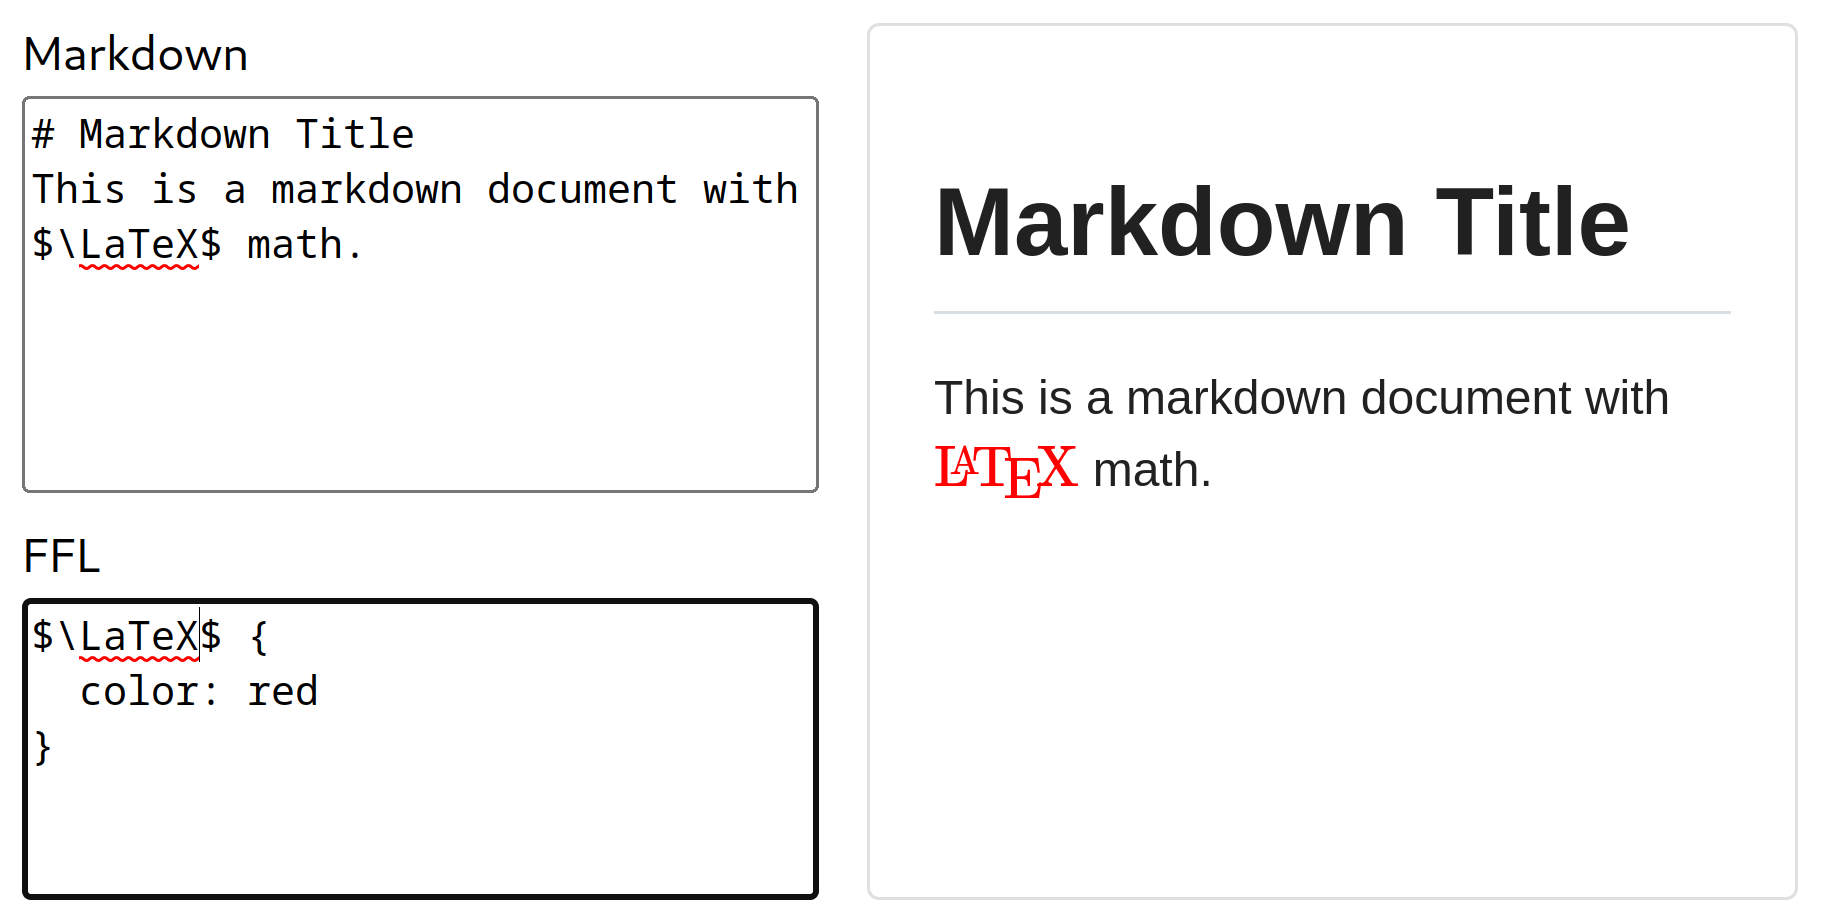
\includegraphics[width=\columnwidth]{md-int.png}
    \caption{Integration with \textit{markdown-it}\cite{MarkdownIt}}
    \label{md}
  \end{figure}
  \vspace*{-1ex}
  It also means that we are not constrained to a single editing environment,
  but rather new environments could be using any web-based technology,
  which has been an enduring and increasingly popular standard
  This way, any \textit{interactivity} can be easily achieved by building tools alongside such
  technologies, and given the variety of different environments that authors might use,
  we provide the opportunity to defer the choice to environment developers,
  and ultimately authors.
  \subsection*{Familiar Syntax}
  Now, despite issues with graphical interfaces, we still need to be careful with the complexity
  of our language. While a complex language would likely allow us to be extremely expressive,
  we still aim for our tool to be relatively \textit{easy to use}. Especially when
  ``clucky syntax''\cite{MAug} is another concern with text-based tools, we intend to minimize
  the learning curve by mirroring chose mirror \LaTeX\ as our syntax of choice for math expressions
  and CSS as our styling language, as both are commonly used and well supoorted
  for their respective purposes on the web. This not only simplifies implementation,
  but it is also our hope that it will create a relatively smooth learning curve
  for any user with experience in either or both. As writing them is already
  likely required to achieve similar effects in most current fashions, this experience
  should not be completely uncommon among authors who might find themselves needing
  styling of math expressions on the web.
  \subsection*{Minimal API}
  Additionally, we restrict our API and responsibilities to processing the input and
  rendering only, mirroring again \textit{KaTeX}'s API so we could serve as
  a drop-in replacement. This should provide our API users\footnote{referring to developers
    who use our implementation to integrate \textit{FFL} with their own editing environments,
    in contrast to users of an authoring environment that might support \textit{FFL},
    which will be referred to more commonly as ``authors''} sufficient flexibility
  in the context of editing environments, minimizing the need for us to intervene to
  implement features for individual environments. For example,
  the possible \textit{interactivity} mentioned above becomes a simple matter of
  calling our API to re-render when the content of the document source has changed.
  \section*{Current Features}
  The overall authoring experience will involve writing both \LaTeX\ math as well
  as \textit{FFL}. The unstyled\footnote{If the input \LaTeX\ has styling elements
    such as \texttt{\textbackslash color}, they will need to be reflected in the selectors
    in this current implementation.} math expression will be written in \LaTeX, and
  all the styling is expected to be done through \textit{FFL}, which
  as of writing supports the following,
  \subsection*{Basic Syntax}
  \textit{FFL} follows a similar format to CSS, in that it is composed of a list
  of ``style rule'' sets, which in turn are a combinations of \textcolor{blue}{selectors}
  and \textcolor{red}{property declarations}, that are global across a single invocation of our rendering
  API. A single style rule block generally looks like the following,
  \begin{align*}
     & \textcolor{blue}{\texttt{\$\textbackslash LaTeX\$}\ \cdots}\ \texttt{\{} \\
     & \ \ \ \ \textcolor{red}{\texttt{color:\;red;}}                           \\
     & \ \ \ \ \textcolor{red}\cdots                                            \\
     & \texttt{\}}
  \end{align*}
  \subsection*{Selectors}
  There are generally two types of selectors, Literal Selectors and Special Classes.
  \subsubsection*{Literal Selectors} are a literal string of \LaTeX\ math expression surrounded by
  a pair of \texttt{\$} as its delimiters, which we have chosen to simplify parsing
  as it is one of the only characters that already cannot be unescaped in \LaTeX\ math mode
  while also being the common delimiters of inline math in general \LaTeX documents.
  Enclosed in the delimiters has no difference from the set of \LaTeX\ math that \textit{KaTeX}
  supports, except for wildcards. As already seen above in Figure \ref{md}, the selector \texttt{\$\textbackslash{LaTeX}\$}
  matches ``\LaTeX'' in the original expression.
  \paragraph*{Wildcards} include \texttt{?} and \texttt{*} which are matches
  single or any number of any token respectively. This is chosen to mirror \texttt{glob}\cite{UnixMan}
  syntax, which is also widely recognized while being much more simplistic compared
  to other language descriptors such as regular expressions.
  This allows us to write more \textit{cross-cutting} selectors.
  As a result, the escaped \texttt{\textbackslash?} and \texttt{\textbackslash*} will now be used
  to match ``?'' and ``*'' is the original math expression.
  For example, \texttt{\$m\_?\$} can match $m_0$ or $m_i$ but not $m_{i,j}$, and
  \texttt{\$f(*)\$} can match $f()$, $f(0)$, $f(x)$, $f(x + 1)$, etc.
  \paragraph*{Special Classes} On top of literal selectors that need to be manually
  written to match parts of the original \LaTeX\ expression, we also pre-configured
  a few commonly used categories of tokens. Note that these are all prefixed by a
  period (\texttt{.}) and we choose to call them ``classes'' to stay within the same
  terminologies as CSS. We currently have the classes below, \\[1ex]
  \begin{tabularx}{\columnwidth}{l|X}
    \textbf{Class Name}   & \textbf{Example \textcolor{blue}{Matches}}                                 \\\hline
    \texttt{.constant}    & $\textcolor{blue}{0}$, $\textcolor{blue}{1}$, $\cdots$                     \\[2pt]
    \texttt{.superscript} & $x^{\textcolor{blue}{0}}$, $e^{\textcolor{blue}{i\pi}}$, $\cdots$          \\[2pt]
    \texttt{.subscript}   & $m_{\textcolor{blue}{0}}$, $n_{\textcolor{blue}{k}}$, $\cdots$             \\[2pt]
    \texttt{.numerator}   & $\frac{\textcolor{blue}{1}}{2}$, $\frac{\textcolor{blue}{k}}{m}$, $\cdots$ \\[2pt]
    \texttt{.denominator} & $\frac{1}{\textcolor{blue}{2}}$, $\frac{k}{\textcolor{blue}{m}}$, $\cdots$ \\
  \end{tabularx}
  \paragraph*{Selector Combinators}
  Some of the special classes are the most useful when combined with literal selectors
  or other special selectors. Currently there are two ways of combining selectors.
  \subparagraph*{Intersection}
  Using \texttt{\textbackslash{intersection}(}{\textit{selector1}, \textit{selector2}, \textit{...}}{\texttt{)}},
  we select the intersection of the selections of all the selectors in the list.
  For example, \texttt{intersection(\$x\_?\$, .constant)} will only match constant
  subscript under $x$.
  \subparagraph*{Union}
  Otherwise, comma-separated selectors on the top-level stands for the union of the
  selections. For example, \texttt{\$x\$, \$y\$} matches the entirety of $xyxxy$.
  \\\par
  In our initial testing, these two combinators are generally sufficient in
  disambiguating in most cases.
  \subsection*{Styling}
  For simplicity in implementation and general compatibility with web technologies,\
  we translate \textit{FFL} to a series of CSS specifications. This also means that
  in most cases, we support CSS style properties directly.
  \subsubsection*{CSS-Based Style Properties}
  The most commonly used property is \texttt{color} but we support the inclusion of
  most CSS properties by directly applying them to corresponding HTML elements
  of the \LaTeX\ selection.\footnote{This does create some undesirable behaviors
    with some properties. See \href{limitations}{Limitations/Naïve Implementation of Certain Features}.}
  \subsubsection*{Additional Style Properties}
  \paragraph*{Labels}
  In addition to colors, another commonly used visual design technique is attaching
  labels to elements of the math expression.
  Currently, we use the \texttt{label} property to specify an auto-placed label with
  a leader line to the boundary of the first instance of selected elements. For example,
  the screenshot below is specified by \texttt{.subscript \{ label : sub; \} }.
  \begin{figure}[H]
    \begin{center}
      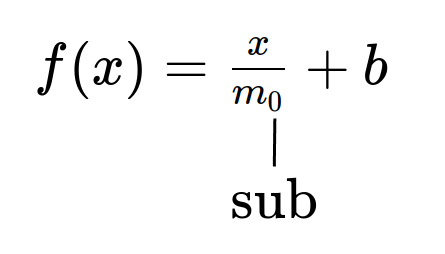
\includegraphics[width=0.5\columnwidth]{label.png}
    \end{center}\vspace*{-1em}
    \caption{Labels}
  \end{figure}
  For the value of the label, we also support \texttt{html( $\cdots$ )}, which
  renders the HTML string directly\footnote{The HTML is sanitized by default, with the potential for configuration}.
  We also by default renders plain (\emph{i.e.} without FFL stylings) \LaTeX\ math inside
  both plain text and HTML labels as we expect it to be commonly useful.
  \subsubsection*{Default Style Refinements}
  Additionally, we do not directly apply some CSS properties but rather handle them
  as special cases due to undesirable default behavior.
  Currently, we support \texttt{background-color} which by default draws background
  for individual text symbols selected, which might have different height and/or baselines.
  Instead, we draw a rectangular box background behind an instance of the selected range
  such that it is clear it is a single selection by our selectors.
  % TODO: Screenshot
  \section*{Implementation Overview}
  In general, we build on top of the \textit{KaTeX} renderer by both preprocessing
  the input \LaTeX\ and its options as well as postprocess its HTML output, while
  mostly relying on \textit{KaTeX}'s engine to process the \LaTeX itself. We choose
  to do this to depend on \textit{KaTeX}'s more robust support and maintenance.
  The pipeline is roughly as follows,
  \subsection*{1. Parsing FFL}
  First we parse FFL using \textit{Peggy}\cite{Peggy}, a PEG parser generator,
  where we define the grammar of our language.
  This allows us to make small modifications to our grammar on demand with minimal effort,
  as surface syntax change is often needed during our iterations.
  \subsection*{2. Matching \& Inserting Marker Tokens}
  With our parsed abstract syntax as the primary data source, we then create a programmatic
  macro afforded by \textit{KaTeX} as part of our calling options, in which we wrap our \LaTeX\
  string during the invocation of its API. At this stage, \textit{KaTeX} will tokenize
  the \LaTeX\ and invoke our macro callback during its expansion, at which point we insert
  special tokens marking the start and end of selection ranges that require styling, which
  will then be passed on to \textit{KaTeX}'s internal HTML representation.
  This is also the point where we determine the escaped CSS class names for our selections
  and transpile all of our styles into a CSS style string.
  After this, we hand off back to \textit{KaTeX} again who will continue to render the
  expanded expression into HTML.
  \subsection*{3. Processing Markers \& Applying Styles}
  After \textit{KaTeX}'s rendering returns, we traverse the DOM tree representation
  in search of previously inserted markers. At the same time during the traversal,
  we apply the escaped CSS classes to the corresponding elements, which we then style
  by inserting previously obtained CSS string as a \texttt{style} element to the DOM
  representation, which could then be converted to an HTML string or the browser's
  representation depending on the API function invoked.
  \subsection*{4. Drawing Additional Overlays}
  Finally, we draw labels and background colors as SVG overlays. Here we locate
  the to-be-styled elements with CSS selectors before finding their bounding box,
  with which we calculate the positions of the background color rectangles as well
  as the positions of their labels with \textit{Labella.js}\cite{Labella}.
  \section*{Preliminary Results}
  So far, we have solicited some informal feedbacks on the tool by asking respondents
  to complete some transcription tasks from rendered equations.
  The results have been so far generally includes suggestions to maintain the liveness
  of our demo environment and general positive reviews of our surface syntax.
  We also found that participants sometimes forget the existence of certain less
  obvious features, despite finding them relatively easy-to-use once reminded.
  For a more formal study, this might mean that we should spend more time introducing
  our features as well as potentially printing out a better cheat sheet.
  \section*{Limitations \& Future Work}\label{limitations}
  In addition to user studies, as is the nature of projects with such a broad design space,
  there are many design decisions we have yet to explore due to limited time in implementation.
  Fortunately, we do believe that many of these feature below, excluding technical limitations,
  range from easy to feasible with reasonable effort on top our current implementation, which we have been
  trying our best to scaffold in a way that should hopefully allow such expansions and refinements.
  \subsection*{Naïve Implementation of Certain Features}
  First among these is to continue delivering on our objective of ``good defaults.''
  As mentioned above, we had to use a custom implementation of \texttt{background-color}
  as the default CSS behavior is not desirable as a default. There are other properties
  such as \texttt{background} and \texttt{border} that might require similar treatments,
  as well as others users might encounter that we have not yet identified.
  \subsection*{Additional Customizations}
  Next on the list is the richer customizations. Even though we aim to provide
  good defaults, some desired refinements have not yet been implemented or for
  which the desired behavior might vary greatly. For example, we plan to attach
  additional classes to the labels to facilitate additional CSS styling, which
  should be an easy feature to implement. And we are considering syntax for
  extent labels as replacement for \texttt{\textbackslash overbrace} and \texttt{\textbackslash underbrace}.
  However, the automatic placement might not be easily feasible without additional
  input flags from the user.
  \subsection*{Scoping}
  As of writing, it is already possible for tool builders to manage their own scoping
  mechanisms by calling our APIs with different styling specifications.
  On the other hand, it could still be potentially useful to allow applying of styles within a limited
  scope within the expression, as currently all styles are invocation-global and
  selector combinators is the main mechanism for disambiguation between contexts
  of identical symbols.
  \subsection*{Pre-Built Integrations}
  As shown earlier, we already have a proof-of-concept implementation of a \textit{markdown-it}
  plugin to render FFL-styled math inside Markdown documents. However, on the way to
  becoming a fully-fledged tool, we might wish to consider integration with more
  commonly used editing environments and architecture our system accordingly.
  \subsection*{Surface Syntax Agnostic API}
  And the interfaces for integration could have great variations. During a conversation
  with Dr. Rowan Cockett at Curvenote, he discussed that FFL-like interactions could
  potentially fit into specifications such as \textit{MyST}\cite{MyST}, though it might
  wish to use its internally consistent syntax. This is likely easy to implement,
  as we would just need to provide a schema for parsed FFL data, which our current
  parser already follows.
  \subsection*{Decisions on Syntax Choices}
  While the syntax might not seem as critical given the consideration of the potential
  for syntax agnostic uses. It would still be useful in evaluating the usefulness of
  our design to provide as universally helpful of a set of syntax as we can, in the case
  that some authors or other users might wish to use the tool ``as-is'' rather than
  relying on developers of editing tools. We should evaluate the ease of our tool
  with use of a thoughtfully designed surface syntax in order to make some of the
  involved decisions.
  \subsection*{Richer Selector Features}
  A central area around our syntax design is the selectors.
  Some might argue ``intersection'' combinators might not be the most intuitive
  way of disambiguating, while other solutions such as lookahead/lookbehind or
  the full CSS style combinators would also introduce a fair amount of complexity.
  While we think selectors has the potential to be feature-ful, the different design
  directions of this remains to be evaluated in order not to obstruct the ease of
  simple tasks.
  \subsection*{Accessibility}
  A lot of math augmentations use expressive colors, and indeed it is also one of
  the scenarios where our tool is the most useful. It might be of concern that this creates
  challenges for visually impaired readers if author over-depend on such augmentations.
  \subsection*{Support for Traditional \LaTeX\ Environments}
  Our tool is built on web technologies, which gives it a tremendous amount of flexibility
  and portability. However, we are unable to address one major use case of an augmentation
  tool, which is offline \LaTeX\ environments often required to produce PDFs, such as
  for scientific paper writing. Although these users tend to already be familiar with
  existing \LaTeX\ toolings such as \textit{tikz}, it is still worth mentioning that it would
  require a considerable amount of effort to re-create similar features in environments
  such as \texttt{pdflatex}.
  \subsection*{Server-Side Rendering of Size-Sensitive Custom Attributes}
  Finally, a current technical limitation, although integration with existing tools
  should overall be relatively straightforward, we did run into issues with editor
  environments that use server-side rendering, such as \textit{VS Code}. In the case
  of server-side rendering, we are unable to obtain the rendered sizes of symbols
  in order to calculate the positions of labels and background. The workarounds that
  have been considered include attaching a headless browser which would significantly
  increase the size of our distributed library, and attaching a deferred script tag to
  the rendered output which would need significant security clearance inside the target
  environment and thus is disabled already in most such environments. Currently,
  we do not render calculated SVG overlays if the tool is used on the server side.
  However, we do not yet consider this issue of high priority as we expect most 
  scenarios that would require rendering of math expressions should have some access
  to the client-side browser.
  \section*{Conclusion}
  Despite much desire for more features and refinements, preliminary results do
  show that FFL could grow into a useful tool that simplifies styling of math
  expressions. As we continue to refine the implementation from our minimum viable
  product, we see many of these features within reach, even if not immediately approached.
  We will also conduct some basic formal user studies to inform said refinements
  in our design in the same process.
  \section*{Additional Acknowledgments}
  We thank Dr. Rowan Cockett for sharing his experience in scientific communication
  and document editing tools, \textit{Penn HCI} lab members for providing feedbacks
  on the tool and many open source contributors that not only created
  the libraries and toolings that we directly cited, but also many indirect dependencies
  that we have used that are so generously shared with everyone.
\end{multicols*}
  \bibliography{refs}
\end{document}
